% =====================================================================
%  CS 6330 - Introduction to Data Science
%  Homework 1: Fast-Food Nutrition
%  Author: Taek Lim
%
%  Build:  latexmk -pdf hw1_taeklim_report.tex
%      or: pdflatex hw1_taeklim_report.tex   (run twice for references)
%
%  Figure paths are relative to this file: ../figures/*.png
% =====================================================================
\documentclass[11pt]{article}

\usepackage[letterpaper,margin=0.75in]{geometry}
\usepackage[T1]{fontenc}
\usepackage[utf8]{inputenc}
\usepackage{amsmath}
\usepackage{array}        % >{...} column modifiers
\usepackage{booktabs}     % \toprule \midrule \bottomrule
\usepackage{float}      % [H] = put the float exactly here, no deferring
\usepackage{graphicx}
\usepackage{caption}
\usepackage{listings}
\usepackage{xcolor}
\usepackage[hidelinks]{hyperref}

\lstset{
  basicstyle=\ttfamily\small,
  breaklines=true,
  frame=single,
  rulecolor=\color{gray!40},
  backgroundcolor=\color{gray!5},
  showstringspaces=false,
  columns=fullflexible,
}

\captionsetup{font=small, labelfont=bf}

% Question heads: sky blue, bold. Darkened from a literal "sky blue" so the
% heading still reads on paper and in greyscale print.
\definecolor{headblue}{HTML}{0C6FB8}
\newcommand{\question}[2]{%
  \section*{\color{headblue}#1 \hfill \normalfont\small(#2)}}


\title{\textbf{Homework 1: Fast-Food Nutrition}\\[2pt]
       \large Descriptive statistics and data manipulation}
\author{Taek Lim \\ \small CS 6330: Introduction to Data Science}
\date{\today}

\begin{document}
\maketitle

\noindent
\textbf{Data.} \texttt{Fast foods - Nutritional information.xlsx} (126 menu items).\\
\textbf{Tooling.} Python 3 / pandas / matplotlib; analysis code written by hand,
all statistics computed programmatically, none typed by hand; figure code written with
Claude Code; ideation manual throughout, including which figures to draw and what
each one should show; write-up drafted with Claude Code.

\vspace{1em}\hrule\vspace{1em}

% =====================================================================
\question{Question 1: Understand the dataset}{15 pts}

\subsection*{Shape and coverage}
\begin{table}[H]\centering\small
\begin{tabular}{l r p{9.2cm}}
\toprule
Measure & Count & Values \\
\midrule
Observations       & 126 & menu items (rows) \\
Variables          & 8   & columns (see Table~\ref{tab:dtypes}) \\
Unique restaurants & 12  & McDonald's, Burger King, Wendy's, Chick-fil-A,
                          Jack in the Box, Sonic, Dairy Queen, Carl's Jr.,
                          Hardee's, White Castle, Whataburger, In-N-Out Burger \\
Unique food types  & 6   & Burger, Milkshake, Breaded Chicken Sandwich,
                          Grilled Chicken Sandwich, Chicken Nuggets, French Fries \\
Missing values     & 0   & none in any of the 8 columns \\
\bottomrule
\end{tabular}
\caption{Shape and coverage of the dataset.}
\end{table}

\subsection*{Data type of each variable}
\begin{table}[H]\centering\small
\begin{tabular}{lll}
\toprule
Variable & Data type & Attribute type \\
\midrule
restaurant    & str     & Categorical, nominal \\
item          & str     & Categorical, nominal \\
type          & str     & Categorical, nominal \\
serving\_size & int64   & Numeric, ratio \\
calories      & int64   & Numeric, ratio \\
fat           & float64 & Numeric, ratio \\
sodium        & int64   & Numeric, ratio \\
sugars        & float64 & Numeric, ratio \\
\bottomrule
\end{tabular}
\caption{Variable types. The three categorical variables are nominal: their values can be
tested only for equality, and reordering the restaurants or food types would change
nothing. The five numeric variables are ratio-scaled, because zero marks the absence of
the quantity, so both differences and ratios are meaningful: an 800\,kcal item really does
carry twice the energy of a 400\,kcal one. None of them is interval-scaled, which would
require an arbitrary zero. Integer storage does not make a variable discrete either:
serving size, calories and sodium are continuous measurements recorded to the nearest unit.}
\label{tab:dtypes}
\end{table}

\subsection*{Descriptive statistics}
\begin{table}[H]\centering\small
\begin{tabular}{l r r r r}
\toprule
 & serving\_size (g) & calories (kcal) & sodium (mg) & sugars (g) \\
\midrule
count   & 126    & 126    & 126     & 126   \\
mean    & 224.27 & 532.49 & 973.75  & 13.29 \\
std     & 108.03 & 250.84 & 523.41  & 21.02 \\
min     & 44     & 130    & 50      & 0     \\
25\%    & 126.50 & 330    & 569.25  & 3     \\
median  & 217.50 & 515    & 930     & 7     \\
75\%    & 315.25 & 670    & 1285.25 & 11    \\
max     & 467    & 1240   & 2460    & 93    \\
IQR     & 188.75 & 340    & 716.00  & 8     \\
skew    & 0.24   & 0.65   & 0.42    & 2.71  \\
\bottomrule
\end{tabular}
\caption{Descriptive statistics for the four quantitative variables.
The skewness row decides which centre to trust: mean and standard deviation are
appropriate where $|\text{skew}| < 1$; for \texttt{sugars} the mean (13.29) sits
\emph{above} the 75th percentile (11), so median and IQR are the honest summary.}
\end{table}

\subsection*{Mode}
\begin{table}[H]\centering\small
\begin{tabular}{l l r r}
\toprule
Variable & Mode(s) & Occurrences & Share of 126 \\
\midrule
serving\_size & 113\,g                         & 4      & 3.2\% \\
calories      & 380, 560, 580, 750 kcal (tied) & 4 each & 3.2\% each \\
sodium        & 1220\,mg                       & 4      & 3.2\% \\
sugars        & 0\,g                           & 17     & 13.5\% \\
\bottomrule
\end{tabular}
\caption{Modal values, with the number of items taking each.}
\end{table}

% \begin{figure}[H]\centering
%   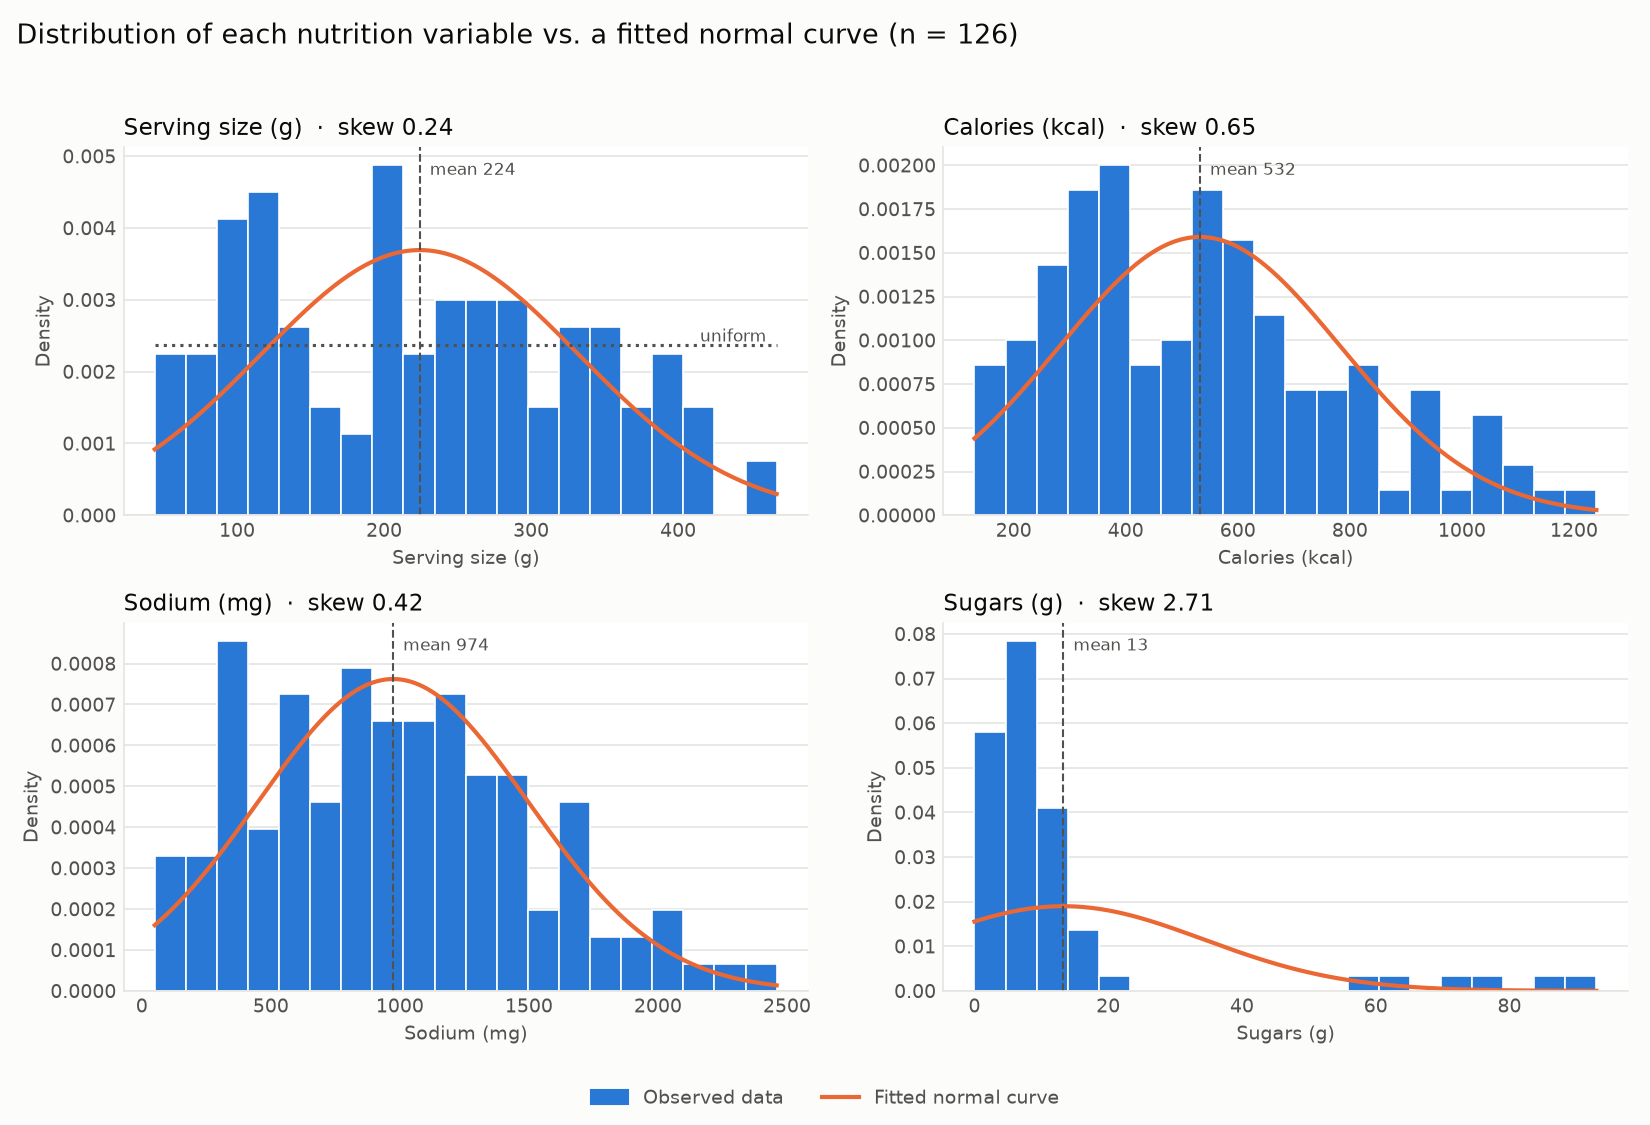
\includegraphics[width=\linewidth]{../figures/fig1_histograms.png}
%   \caption{Histograms of the four quantitative variables with a normal curve fitted
%   from the sample mean and standard deviation. \texttt{serving\_size} is near-symmetric
%   but flat rather than bell-shaped; \texttt{calories} and \texttt{sodium} are
%   single-peaked with a mild right tail, so a normal approximation is workable;
%   \texttt{sugars} is nowhere near normal, since the fitted curve places mass at 30 to 50\,g
%   where the data has none.}
% \end{figure}

% \begin{figure}[H]\centering
%   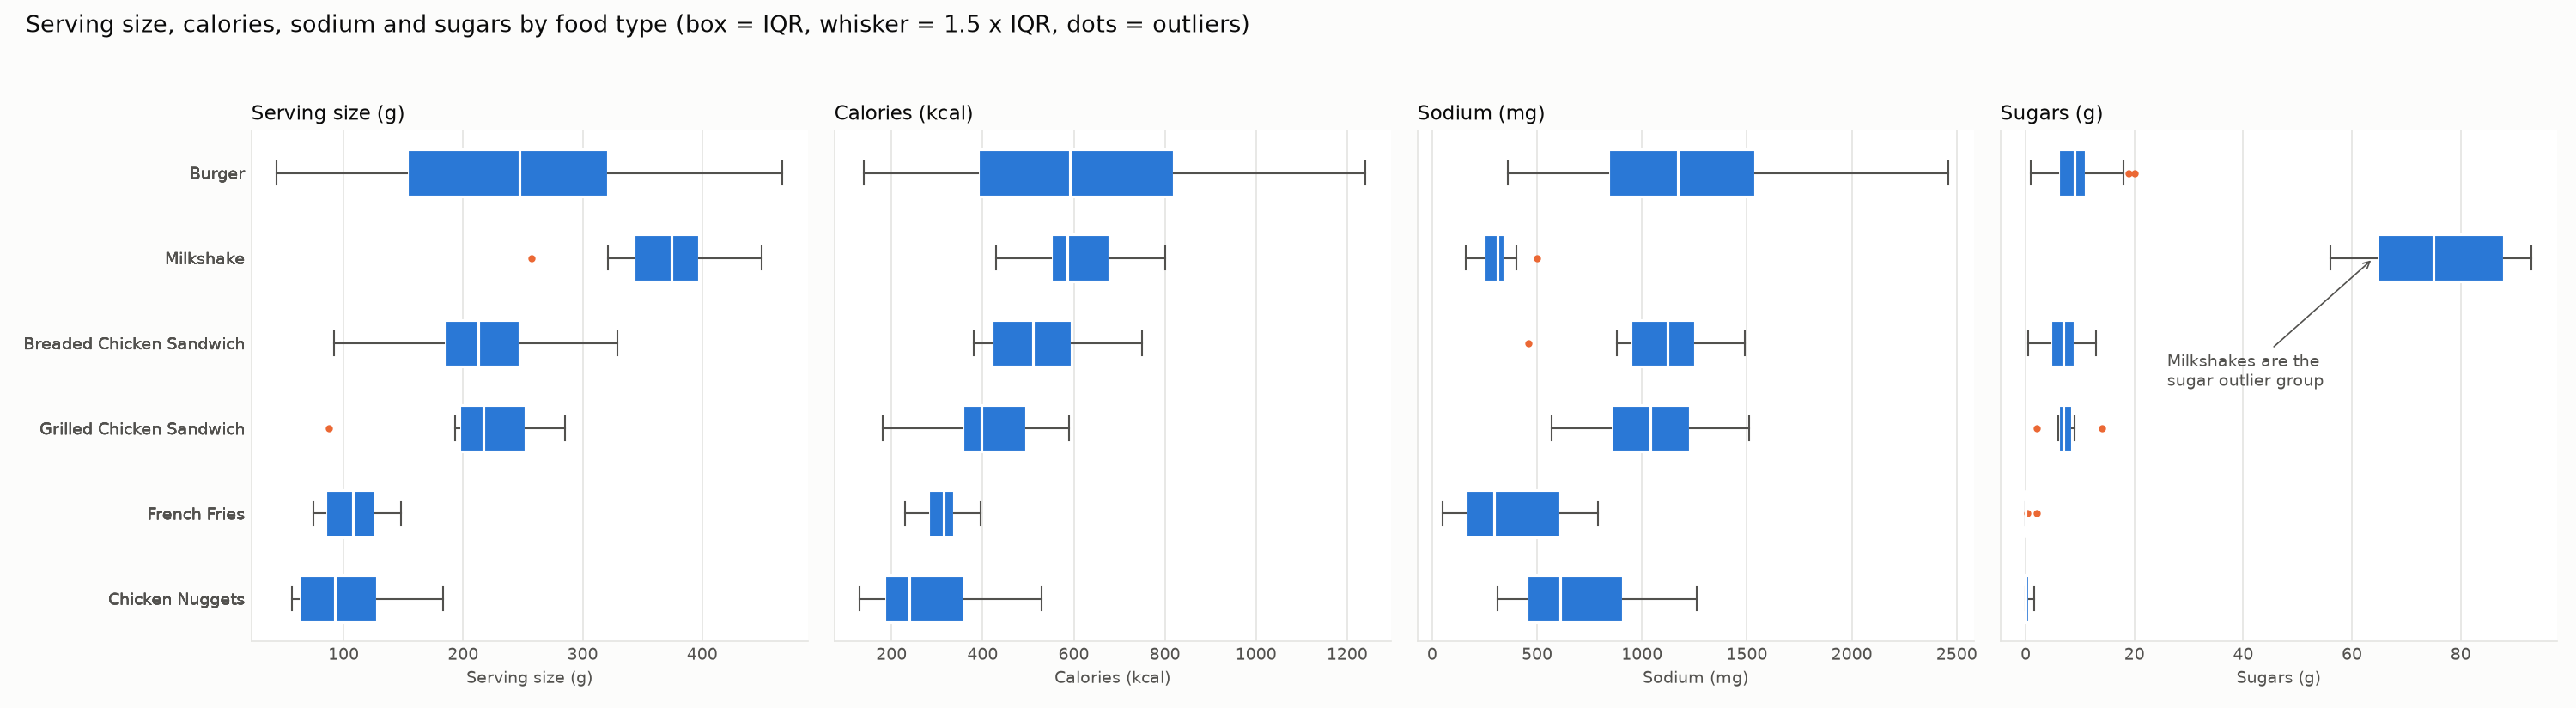
\includegraphics[width=\linewidth]{../figures/fig2_boxplot_by_type.png}
%   \caption{All four quantitative variables by food type (box = IQR, whiskers reach the last
%   observation within $1.5\times$IQR of the box, dots = outliers). Calories rise monotonically
%   from Chicken Nuggets to Burger, and sodium runs the opposite way from sugars: burgers and
%   both chicken sandwiches sit above 1000\,mg of sodium while the milkshakes carry the sugar.
%   Serving size does not track any of them. A milkshake is the heaviest item on the menu at a
%   median 374.5\,g, yet it delivers roughly the same energy (median 585\,kcal) as a 247\,g
%   burger (median 591\,kcal), so weight alone predicts nothing about what is inside.}
%   \label{fig:box}
% \end{figure}

\begin{figure}[H]\centering
  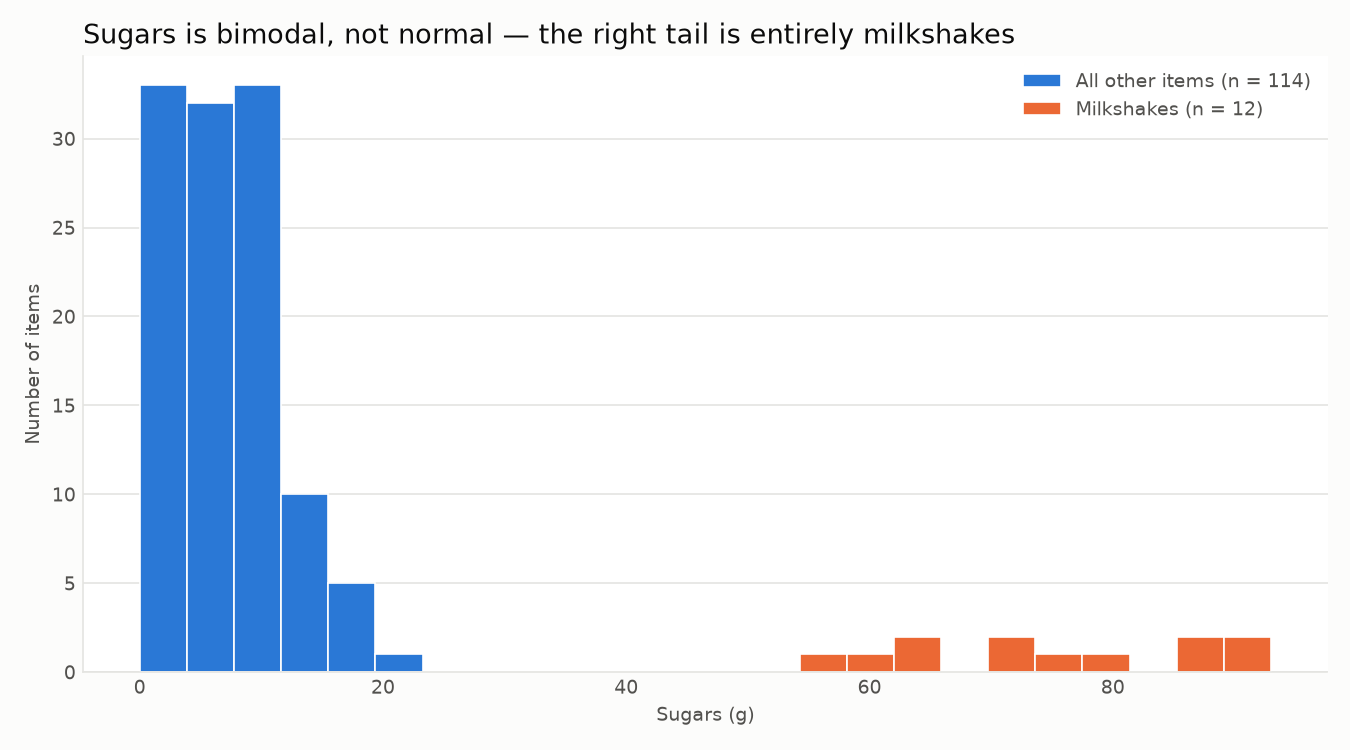
\includegraphics[width=0.85\linewidth]{../figures/fig3_sugars_bimodal.png}
  \caption{Why \texttt{sugars} is skewed. Splitting by food type shows the 2.71 skew is
  not a long tail but \emph{two separate populations}: 114 items at 0 to 20\,g and
  12 milkshakes at 56 to 93\,g, with no observation at all between 20 and 56\,g.}
  \label{fig:sugars}
\end{figure}

\subsection*{What I learned}
About the data:
\begin{itemize}
  \item The dataset is complete. It holds 126 records across 12 restaurants and 6 food
        types, with no missing values. A \texttt{sugars} reading of 0\,g is a real
        measurement, not a gap.
  \item The spread is wide. In every quantitative variable the standard deviation is at
        least half the mean (48\%, 47\%, 54\% and 158\% of the mean), so no variable
        sits close to its centre.
  \item \texttt{sugars} is skewed. Its mean is 13.29\,g but the 75th percentile is only
        11\,g, so a few large values pull the mean above three quarters of the data.
        Figure~\ref{fig:sugars} shows the cause: the distribution is bimodal.
\end{itemize}

\noindent
About the tools: I learned how to pin a Python version for a project and work inside a
virtual environment, and how to use pandas to describe a dataset. I also learned that a
chart is often the faster way to explain a result, since the shape of \texttt{sugars}
is obvious in a histogram and invisible in a table of means.

% =====================================================================
\clearpage
\question{Question 2: Find extreme observations}{12 pts}

\subsection*{Five highest-sodium items}
\begin{table}[H]\centering\small
\begin{tabular}{llrrl}
\toprule
Restaurant & Item & Sodium (mg) & Calories & Type \\
\midrule
Hardee's        & 2/3 LB Double Thickburger      & 2460 & 1140 & Burger \\
Hardee's        & 1/2 LB Original Thickburger    & 2240 & 1030 & Burger \\
Jack in the Box & Bacon Ultimate Cheeseburger    & 2190 & 910  & Burger \\
Whataburger     & A.1. Thick \& Hearty Burger    & 2080 & 990  & Burger \\
Wendy's         & 3/4 lb. Triple w/ Cheese       & 1990 & 1090 & Burger \\
\bottomrule
\end{tabular}
\caption{Sorted highest to lowest sodium. All five are burgers. Item names are reproduced
from the source file with two spelling corrections (\texttt{Thinkbuger} $\rightarrow$
Thickburger) and trademark symbols dropped; all numbers are unaltered.}
\end{table}

\subsection*{Minimum- and maximum-calorie items (all eight variables)}
\begin{table}[H]\centering\footnotesize\setlength{\tabcolsep}{4pt}
\begin{tabular}{l l >{\raggedright\arraybackslash}p{3.4cm} l r r r r r}
\toprule
 & Restaurant & Item & Type & Serving (g) & Calories & Fat (g) & Sodium (mg) & Sugars (g) \\
\midrule
Min & Chick-fil-A & Chicken Nuggets (4pc) & Chicken Nuggets & 57 & 130 & 6.0 & 545 & 1.5 \\
Max & Sonic & SuperSonic Bacon Double CheeseBurger w Mayo & Burger & 396 & 1240 & 87.0 & 1690 & 8.0 \\
\bottomrule
\end{tabular}
\caption{Complete records (all eight variables) for the minimum- and maximum-calorie items.}
\end{table}

\subsection*{Why complete records are more informative}
Reporting the complete record lets me compare the calorie extremes on calories per gram
rather than raw calories: 1240\,kcal / 396\,g $\approx$ 3.13\,kcal/g versus 130\,kcal /
57\,g $\approx$ 2.28\,kcal/g. The maximum item has 9.54 times the calories but only about
1.4 times the calories per gram, so most of the difference comes from portion size
(396\,g versus 57\,g), and the \texttt{fat} variable shows that roughly 63\% of its 1240
calories comes from fat alone. The five-variable sodium table omits \texttt{serving\_size},
so those items cannot be compared per gram, which is exactly the information that a
complete record preserves.

% =====================================================================
\clearpage
\question{Question 3: Filter with multiple conditions}{12 pts}

\subsection*{Subset count}

Subset condition: \texttt{calories < 500 AND sodium < 1000}, applied as a single mask so
both conditions must hold for the same item. \textbf{Qualifying items: 49} of 126.
Taken separately, 60 items have fewer than 500 calories and 68 have less than 1000\,mg
sodium, so the joint condition is what reduces the subset to 49.

\subsection*{Qualifying items by restaurant}

\begin{table}[H]\centering\small
\begin{tabular}{lr}
\toprule
Restaurant & Qualifying items \\
\midrule
Jack in the Box   & 7 \\
White Castle      & 7 \\
McDonald's        & 5 \\
Burger King       & 5 \\
Wendy's           & 5 \\
Carl's Jr.        & 4 \\
Chick-fil-A       & 3 \\
Sonic             & 3 \\
Dairy Queen       & 3 \\
Whataburger       & 3 \\
Hardee's          & 2 \\
In-N-Out Burger   & 2 \\
\bottomrule
\end{tabular}
\caption{Counts sorted highest to lowest.}
\end{table}

\noindent
\textbf{Ties.} Most counts are tied, so all tied restaurants are reported: 7 (Jack in the
Box, White Castle), 5 (McDonald's, Burger King, Wendy's), 3 (Chick-fil-A, Sonic, Dairy Queen,
Whataburger), 2 (Hardee's, In-N-Out Burger); only Carl's Jr.\ at 4 stands alone. Every one of
the 12 restaurants has at least one qualifying item, so no restaurant is missing from the table.

\subsection*{What each row represents}

One restaurant, and the \emph{number of that
restaurant's menu items that satisfy both conditions simultaneously}: fewer than 500
calories \emph{and} less than 1000\,mg sodium. It is a count of items, not of restaurants,
and it is not a rate: a restaurant with a long menu can show a high count without
offering a higher \emph{proportion} of light items.

% =====================================================================
\clearpage
\question{Question 4: Summarize by food type}{15 pts}

\subsection*{Item counts and calorie statistics by food type}

One row per food type, giving the number of menu items (\texttt{n}) and the mean, standard
deviation, minimum, and maximum of \texttt{calories}. The SD is the sample standard
deviation (\texttt{ddof=1}), which is what \texttt{pandas} reports by default in
\texttt{describe()} and \texttt{std()}.

\begin{table}[H]\centering\small
\begin{tabular}{lrrrrr}
\toprule
Food type & n & Mean & SD & Min & Max \\
\midrule
Burger                   & 69 & 620.20 & 277.16 & 140 & 1240 \\
Milkshake                & 12 & 606.67 & 98.84  & 430 & 800  \\
Breaded Chicken Sandwich & 11 & 522.09 & 117.04 & 380 & 750  \\
Grilled Chicken Sandwich & 11 & 408.00 & 124.02 & 180 & 590  \\
French Fries             & 12 & 314.08 & 49.69  & 230 & 395  \\
Chicken Nuggets          & 11 & 274.55 & 119.78 & 130 & 530  \\
\bottomrule
\end{tabular}
\caption{Calories by food type, sorted highest to lowest mean. Sample SD (\texttt{ddof=1}).}
\end{table}

\begin{table}[H]\centering\small
\begin{tabular}{lrrrrr}
\toprule
 & n & Mean & SD & Min & Max \\
\midrule
Overall & 126 & 532.49 & 250.84 & 130 & 1240 \\
\bottomrule
\end{tabular}
\caption{Calories over all 126 items pooled.}
\end{table}

\subsection*{Two observations}

\paragraph{Observation 1.} Burgers have the highest mean calories (620.20), but they are
also the most widely spread type, with a standard deviation of 277.16 and a range from 140
to 1240 calories. Because the spread is this large, knowing only that an item is a burger
does not tell me much about its calorie count.

\paragraph{Observation 2.} Milkshakes average almost as high as burgers (606.67 vs.\ 620.20,
a gap of 13.53) but with a third of the variability (SD 98.84 vs.\ 277.16, range 430 to 800).
A milkshake is \emph{reliably} calorie-dense, whereas a burger may be light (140) or
extreme (1240). The two means are close; the two distributions are not.

% =====================================================================
\clearpage
\question{Question 5: Summarize by restaurant}{15 pts}

\subsection*{Menu items and mean calories, sodium, and sugars by restaurant}

\begin{table}[H]\centering\small
\begin{tabular}{lrrrr}
\toprule
Restaurant & n & Mean calories & Mean sodium (mg) & Mean sugars (g) \\
\midrule
Hardee's        & 12 & 691.67 & 1399.17 & 14.92 \\
Whataburger     & 12 & 603.33 & 1149.17 & 14.75 \\
Sonic           & 11 & 588.18 & 926.36  & 10.00 \\
Carl's Jr.      & 13 & 585.31 & 1085.92 & 12.99 \\
Wendy's         & 12 & 549.17 & 1057.50 & 14.17 \\
Jack in the Box & 13 & 541.54 & 1082.31 & 11.69 \\
Burger King     & 11 & 540.00 & 817.27  & 14.00 \\
Dairy Queen     & 11 & 516.36 & 1001.82 & 12.09 \\
In-N-Out Burger & 5  & 505.00 & 731.00  & 19.00 \\
McDonald's      & 11 & 441.82 & 766.36  & 12.45 \\
Chick-fil-A     & 5  & 330.00 & 654.00  & 18.50 \\
White Castle    & 10 & 319.00 & 568.00  & 10.60 \\
\bottomrule
\end{tabular}
\caption{Sorted by mean calories, highest to lowest.}
\end{table}

\subsection*{Highest and lowest restaurant on each mean measure}

\begin{itemize}\itemsep2pt
  \item \textbf{Mean calories:} highest = Hardee's (691.67), lowest = White Castle (319.00).
  \item \textbf{Mean sodium:} highest = Hardee's (1399.17), lowest = White Castle (568.00).
  \item \textbf{Mean sugars:} highest = In-N-Out Burger (19.00), lowest = Sonic (10.00).
\end{itemize}

\subsection*{Why these summaries are not comparisons of equivalent menus}

These means describe only the items from each restaurant that are in this dataset, not the
whole menu, and the menus are not made up of the same things: Chick-fil-A has no burger
here, so its low mean (330.00) mostly shows that the highest-calorie food type is missing
from its list, not that its food is lighter. The number of items also differs a lot, from 5 for In-N-Out Burger to
13 for Carl's Jr., so a mean based on only 5 items is much less reliable than one based on
13. To compare restaurants fairly, I would have to compare the same food type across
restaurants.

% =====================================================================
\clearpage
\question{Question 6: Use two grouping variables}{23 pts}

\subsection*{Mean calories for every restaurant $\times$ food-type combination, and the lowest-mean restaurant in each type}
\begin{table}[H]\centering\footnotesize\setlength{\tabcolsep}{2pt}
\begin{minipage}{0.49\textwidth}\centering
\begin{tabular}{llrr}
\toprule
Food type & Restaurant & Mean cal. & n \\
\midrule
Breaded Chicken Sandwich & In-N-Out Burger & 0.00 & 0 \\
Breaded Chicken Sandwich & White Castle & 380.00 & 1 \\
Breaded Chicken Sandwich & Chick-fil-A & 410.00 & 1 \\
Breaded Chicken Sandwich & Jack in the Box & 410.00 & 1 \\
Breaded Chicken Sandwich & Whataburger & 430.00 & 1 \\
Breaded Chicken Sandwich & Carl's Jr. & 493.00 & 1 \\
Breaded Chicken Sandwich & McDonald's & 510.00 & 1 \\
Breaded Chicken Sandwich & Wendy's & 510.00 & 1 \\
Breaded Chicken Sandwich & Sonic & 580.00 & 1 \\
Breaded Chicken Sandwich & Dairy Queen & 610.00 & 1 \\
Breaded Chicken Sandwich & Burger King & 660.00 & 1 \\
Breaded Chicken Sandwich & Hardee's & 750.00 & 1 \\
Burger & Chick-fil-A & 0.00 & 0 \\
Burger & White Castle & 244.00 & 5 \\
Burger & McDonald's & 508.33 & 6 \\
Burger & In-N-Out Burger & 513.33 & 3 \\
Burger & Dairy Queen & 571.67 & 6 \\
Burger & Jack in the Box & 590.00 & 8 \\
Burger & Burger King & 626.67 & 6 \\
Burger & Wendy's & 662.86 & 7 \\
Burger & Carl's Jr. & 686.75 & 8 \\
Burger & Sonic & 690.00 & 6 \\
Burger & Whataburger & 738.57 & 7 \\
Burger & Hardee's & 804.29 & 7 \\
Chicken Nuggets & In-N-Out Burger & 0.00 & 0 \\
Chicken Nuggets & Chick-fil-A & 130.00 & 1 \\
Chicken Nuggets & Burger King & 170.00 & 1 \\
Chicken Nuggets & Wendy's & 180.00 & 1 \\
Chicken Nuggets & McDonald's & 190.00 & 1 \\
Chicken Nuggets & Carl's Jr. & 220.00 & 1 \\
Chicken Nuggets & Jack in the Box & 240.00 & 1 \\
Chicken Nuggets & Hardee's & 260.00 & 1 \\
Chicken Nuggets & Dairy Queen & 350.00 & 1 \\
Chicken Nuggets & Whataburger & 370.00 & 1 \\
Chicken Nuggets & Sonic & 380.00 & 1 \\
Chicken Nuggets & White Castle & 530.00 & 1 \\
\bottomrule
\end{tabular}
\end{minipage}\hfill
\begin{minipage}{0.49\textwidth}\centering
\begin{tabular}{llrr}
\toprule
Food type & Restaurant & Mean cal. & n \\
\midrule
French Fries & McDonald's & 230.00 & 1 \\
French Fries & Sonic & 250.00 & 1 \\
French Fries & Chick-fil-A & 280.00 & 1 \\
French Fries & Whataburger & 280.00 & 1 \\
French Fries & Carl's Jr. & 304.00 & 1 \\
French Fries & Wendy's & 310.00 & 1 \\
French Fries & Burger King & 320.00 & 1 \\
French Fries & Jack in the Box & 330.00 & 1 \\
French Fries & White Castle & 330.00 & 1 \\
French Fries & Hardee's & 360.00 & 1 \\
French Fries & Dairy Queen & 380.00 & 1 \\
French Fries & In-N-Out Burger & 395.00 & 1 \\
Grilled Chicken Sandwich & In-N-Out Burger & 0.00 & 0 \\
Grilled Chicken Sandwich & White Castle & 180.00 & 1 \\
Grilled Chicken Sandwich & Chick-fil-A & 270.00 & 1 \\
Grilled Chicken Sandwich & McDonald's & 350.00 & 1 \\
Grilled Chicken Sandwich & Dairy Queen & 360.00 & 1 \\
Grilled Chicken Sandwich & Wendy's & 370.00 & 1 \\
Grilled Chicken Sandwich & Carl's Jr. & 398.00 & 1 \\
Grilled Chicken Sandwich & Burger King & 420.00 & 1 \\
Grilled Chicken Sandwich & Sonic & 450.00 & 1 \\
Grilled Chicken Sandwich & Jack in the Box & 540.00 & 1 \\
Grilled Chicken Sandwich & Whataburger & 560.00 & 1 \\
Grilled Chicken Sandwich & Hardee's & 590.00 & 1 \\
Milkshake & Whataburger & 430.00 & 1 \\
Milkshake & McDonald's & 530.00 & 1 \\
Milkshake & Dairy Queen & 550.00 & 1 \\
Milkshake & White Castle & 550.00 & 1 \\
Milkshake & Chick-fil-A & 560.00 & 1 \\
Milkshake & Wendy's & 580.00 & 1 \\
Milkshake & In-N-Out Burger & 590.00 & 1 \\
Milkshake & Burger King & 610.00 & 1 \\
Milkshake & Sonic & 670.00 & 1 \\
Milkshake & Carl's Jr. & 700.00 & 1 \\
Milkshake & Hardee's & 710.00 & 1 \\
Milkshake & Jack in the Box & 800.00 & 1 \\
\midrule
\textbf{Overall} & & \textbf{532.49} & \textbf{126} \\
\bottomrule
\end{tabular}
\end{minipage}
\caption{Mean calories for the full $6 \times 12 = 72$ restaurant $\times$ food-type grid,
sorted by food type and then by mean calories. The four combinations that do not appear in
the menu data are shown as $0.00$ with $n = 0$. The table continues in the right column.}
\end{table}

The four combinations shown as $0$:
\begin{itemize}\itemsep2pt
  \item In-N-Out Burger, Breaded Chicken Sandwich
  \item In-N-Out Burger, Grilled Chicken Sandwich
  \item In-N-Out Burger, Chicken Nuggets
  \item Chick-fil-A, Burger
\end{itemize}

Within each food type the minimum of those means is taken, and every restaurant attaining it
is returned (see \emph{Tie handling} below).

\subsection*{Lowest mean calories per food type (six rows)}
\begin{table}[H]\centering\small
\begin{tabular}{llrr}
\toprule
Food type & Restaurant & Mean calories & n items \\
\midrule
Breaded Chicken Sandwich & White Castle & 380.00 & 1 \\
Burger                   & White Castle & 244.00 & 5 \\
Chicken Nuggets          & Chick-fil-A  & 130.00 & 1 \\
French Fries             & McDonald's   & 230.00 & 1 \\
Grilled Chicken Sandwich & White Castle & 180.00 & 1 \\
Milkshake                & Whataburger  & 430.00 & 1 \\
\bottomrule
\end{tabular}
\caption{Lowest mean calories per food type. Note the $n$ column: five of the six
``winners'' rest on a single menu item, so only the Burger row (White Castle, $n=5$)
is a stable estimate.}
\end{table}

\subsection*{Tie handling}
My procedure finds the minimum mean within each food type and returns every restaurant whose
mean is equal to that minimum. Three ways of doing this give the same six rows on this
dataset:
\begin{lstlisting}[language=Python]
1. g.loc[g.groupby("type").mean_cal.idxmin()]
2. g.sort_values("mean_cal").groupby("type").head(1)
3. g[g.mean_cal == g.groupby("type").mean_cal.transform("min")]
\end{lstlisting}

\noindent The first two keep only one row per food type, so if two restaurants had the same
lowest mean, one of them would be dropped without any error message. The third one compares
every mean against the group minimum, so it returns all tied restaurants and the table would
have more than six rows. No tie occurs in this dataset, so all three happen to be correct
here, but on a larger dataset ties do happen, and silently dropping a tied record means
losing information and possibly making a decision based on an incomplete answer. That is why
I used the third method.

% =====================================================================
\clearpage
\question{Question 7: Debug an analysis}{8 pts}

\subsection*{Mean calories for every restaurant}
\begin{table}[H]\centering\small
\begin{tabular}{lr}
\toprule
Restaurant & Mean calories \\
\midrule
Hardee's & 691.67 \\
Whataburger & 603.33 \\
Sonic & 588.18 \\
Carl's Jr. & 585.31 \\
Wendy's & 549.17 \\
Jack in the Box & 541.54 \\
Burger King & 540.00 \\
Dairy Queen & 516.36 \\
In-N-Out Burger & 505.00 \\
McDonald's & 441.82 \\
Chick-fil-A & 330.00 \\
White Castle & 319.00 \\
\bottomrule
\end{tabular}
\caption{Mean calories by restaurant, highest to lowest. The answer to the question is the
first row of this table.}
\end{table}

\subsection*{Result of the given code}
\begin{lstlisting}[language=Python]
df.groupby('restaurant')['calories'].mean().sort_values().head(1)

restaurant
White Castle    319.00
\end{lstlisting}

\noindent Listing output is rounded to two decimal places throughout, matching the tables.

The R version has the same defect:
\begin{lstlisting}[language=R]
df |>
  group_by(restaurant) |>
  summarise(mean_calories = mean(calories)) |>
  arrange(mean_calories) |>
  slice_head(n = 1)
\end{lstlisting}

\noindent Both return the \emph{last} row of the table above, not the first one. The code
runs without any error message, so the wrong answer is easy to miss.

\subsection*{Corrected code}
\begin{lstlisting}[language=Python]
df.groupby('restaurant')['calories'].mean().sort_values(ascending=False).head(1)
\end{lstlisting}

\begin{lstlisting}[language=R]
df |>
  group_by(restaurant) |>
  summarise(mean_calories = mean(calories)) |>
  arrange(desc(mean_calories)) |>
  slice_head(n = 1)
\end{lstlisting}

\subsection*{Result of the corrected code}
\begin{lstlisting}[language=Python]
restaurant
Hardee's    691.67
\end{lstlisting}

\noindent This matches the first row of the table above.

\subsection*{Why the original code was wrong}
\texttt{sort\_values()} sorts in ascending order by default, so \texttt{head(1)} took the
smallest mean instead of the largest. \texttt{arrange()} in R defaults to ascending in the
same way, so \texttt{slice\_head(n = 1)} has the same problem. Adding
\texttt{ascending=False}, or \texttt{desc()} in R, sorts from highest to lowest, and the
first row is then the restaurant the question asks for. The grouping and the mean were
already correct.

\subsection*{A problem that remains after the fix}
\texttt{head(1)} returns one row no matter what, so if two restaurants had the same highest
mean, one of them would be dropped without any warning. Comparing every mean against the
maximum returns all of them instead, which is the same tie rule I used in Question 6:
\begin{lstlisting}[language=Python]
s = df.groupby('restaurant')['calories'].mean()
s[s == s.max()]
\end{lstlisting}

\begin{lstlisting}[language=R]
df |>
  group_by(restaurant) |>
  summarise(mean_calories = mean(calories)) |>
  filter(mean_calories == max(mean_calories))
\end{lstlisting}

\noindent No tie occurs in this dataset, so this returns exactly one row, Hardee's at 691.67.

\end{document}
